\chapter{Methodology}\label{ch:methodology}

Data Quality methodology consists of two main parts, the model and the metamodel.
The model defines activities, their description, goals and sequence of order needed for extraction of Data Quality metrics.
The metamodel defines components of DQ process, maps the relationship among the components and activities respectively.

\section{Model}

The methodology has several important components that need to be identified or developed.
The metamodel that covers the required components is as depicted in the Figure~\ref{fig:methodology-metamodel}.
The activities within the process model have a goal to develop those components.

Overall, the methodology consists of two main processes.
The first one is \textbf{Specification Process}.
The goal of this processs is to identify and define context specific ways to measure data quality.
The second one is an \textbf{Execution Process}.
Its main goal is to \textit{collect} and \textit{verify} data with output from \textit{Specification Process} taken into account.

\begin{figure}[htb]
    \centering
    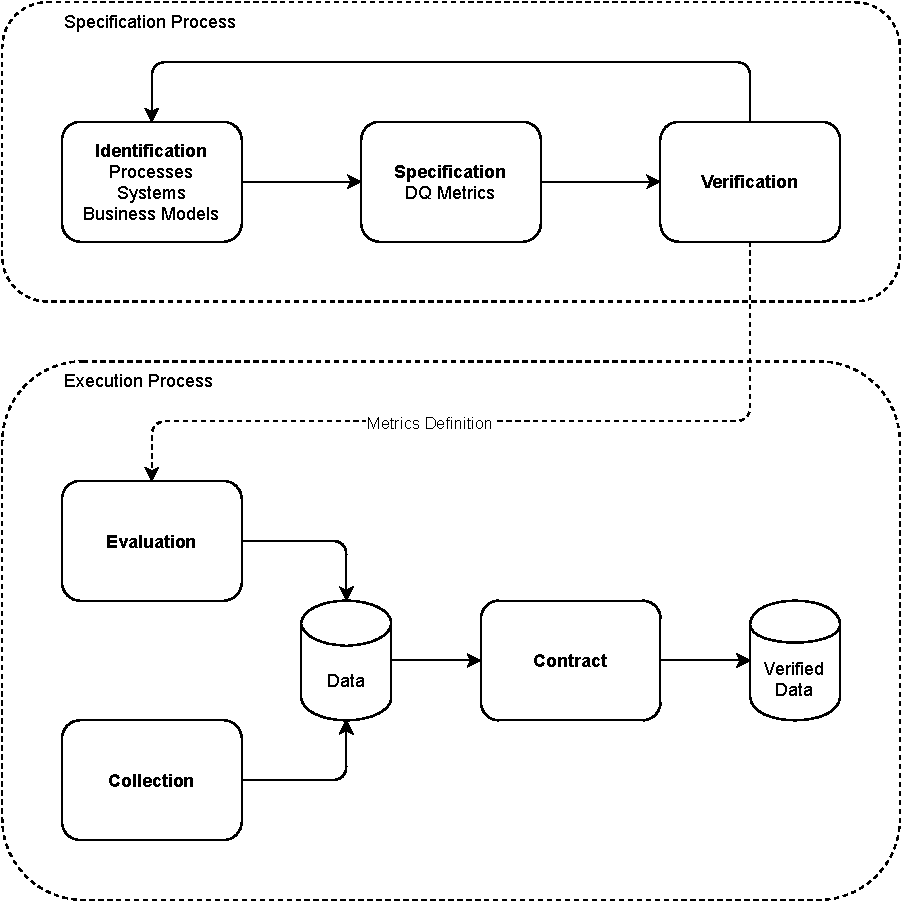
\includegraphics[width=.8\textwidth]{figures/dq-methodology.pdf}
    \caption{Methodology Metamodel}
    \label{fig:methodology-metamodel}
\end{figure}
\FloatBarrier

\subsection{Specification Process}

% Specifikační proces slouží jako nástroj pro definování kvalitativních a kvantifikovatelných požadavků na kvalitu.
The specification process serves as a tool for defining qualitative and quantifiable quality requirements.
This is a key part of the system.
% Je to však také jediná část procesu, která vyžaduje nezbytnou iniciativu analytika či analytického týmu.
However, it is also the only part of the process that requires the necessary initiative of the analyst or analytical team.
Now, we describe each part of the process.

\begin{figure}[htb]
    \centering
    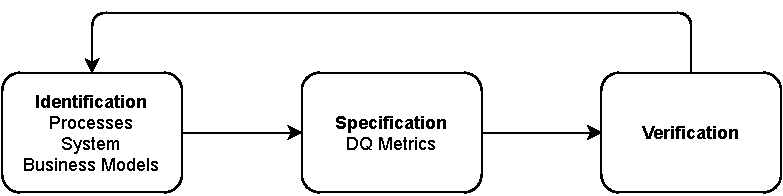
\includegraphics[width=.8\textwidth]{figures/specification-process.pdf}
    \caption{Specification Process}
    \label{fig:specification-process}
\end{figure}
\FloatBarrier

\subsubsection{Identification}

This activity focuses on identification of systems, processes and business schemes generatig data.
By identifying weak points and bottlenecks in those processes, we can find causes of poor data.
Also, we need to identify the subprocesses or activities that are mostly affected by the product data quality.

\subsubsection{Metrics Specification}

The goal of this activity is to identify the process metrics or KPIs.
Measuring data quality is all about understanding what data quality attributes are, and choosing the correct data quality metrics.
A comprehensive list of Data Quality Attributes by Eppler (2006) is available in appendix~\ref{ch:data-quality-attributes}.
Specific attributes will be further discussed in Chapter~\ref{ch:quality-classification-system}.

\subsubsection{Verification}

The last part of current process is verification.
This activity has to ensure that selected metrics are meaningful enough, capturing the actual condition of data.

\subsection{Execution Process}

The second main component is the execution process.
This includes the actual collection and validation of data against the requirements obtained by the analysis from the first process.
Ideally, in a semi-automated information system, this part runs independently, without human intervention.
However, we are aware that in many cases it is not possible to implement a fully automated system, either due to the information complexity of the task or the financial costs of system development.

\begin{figure}[htb]
    \centering
    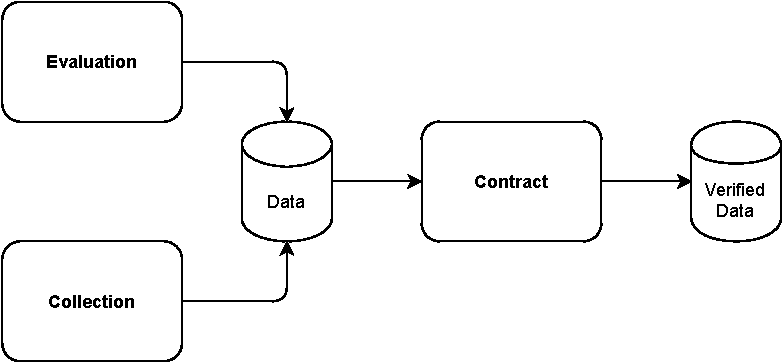
\includegraphics[width=.8\textwidth]{figures/execution-process.pdf}
    \caption{Execution Process}
    \label{fig:execution-process}
\end{figure}
\FloatBarrier

\subsubsection{Collection}

Data collection is a systematic process of gathering observations or measurements.
Data collector can be either \textit{Information System}, computer program or a human.
Before the beginning of collecting data, we need to consider:

\begin{itemize}
    \item the type of data we will collect;
    \item the methods and procedures we will use to collect, store and process data.
\end{itemize}

\subsubsection{Verification}

In our general case, verification is based on actual reliability of data, computed using DQ metrics.
In other scenarios, the verification could be based on data redundancies, therefore based on the comparison of the collected data from two or more different collectors.
If all data match, the data will be considered as valid.
If not, the data remains invalid until a further collector validates it.

Artificial Intelligence and Machine Learning could be used to further ease and optimize data verification.
Especially when processing image data and data with a high level of abstraction.

\subsubsection{Contract}

The contractual process is a subprocess that has the task of marking data as trustworthy if all the necessary requirements are met.
This is the same concept as the so-called \enquote{smart contracts}.
Smart contracts are essentially blockchain programs that are processed when mandatory conditions are fulfilled.
They are commonly used to simplify agreement implementation so that all parties can be sure of the result instantly, without intermediary intervention or time loss.
This leads to workflow automation, initiating the next step if all conditions have been satisfied.

The contracts work by following simple \enquote{if-then} statements.
This mechanism might include allocation of funds to the appropriate parties, sending notifications, or releasing a ticket.

\subsection{Supporting Techniques}

There are a several data quality rules one can deduce from a Feedback-Control Systems view of information systems reviewed by Orr (1998).

\begin{enumerate}
    \item Unused data cannot remain correct for very long;
    \item data quality in an information system is a function of its use, not its collection;
    \item data quality cannot be better than its most strict use;
    \item data quality problems tend to become worse as the system ages;
    \item the less likely some data attribute is to change, the harder it will be to change it when the time comes;
    \item laws of data quality apply equally to data and metadata~\cite{orr1998}.
\end{enumerate}

To prevent the consequences of these rules and the unauthorized creation of data, we present two additianal concepts.
These concepts should be incorporated into the design of the information system respecting the proposed methodology.

\subsubsection{Proof of Constancy}

Proof of Constant Data, alias Proof of Constancy, is a way to assure a constant accuracy of data.
Data have to be regularly updated to keep the accuracy rate high.
Data accuracy rate will decrease progressively based on a specific time frame basis (e.g., X\% per month).
This percentage is different depending on the type of data.
Datasets more sensitive to changes may see this rate decrease by 5\% to 10\% per month or day depending on the circumstances.
On the other hand, established, well-known sets, will see their rate decrease by 0.1\% per month or even year.
A scale of discount rates will have to be established based on the areas of interest and actual items collected.

\subsubsection{Proof of Trust}

Proof of Trust is an instrument for data collector evaluation.
The collector or generator will get \enquote*{quality score} for his/her or its collection actions.
The more collectors initiate, update and verify data correctly, the higher their \enquote*{quality score} will be.
A higher quality score leads to a higher level of \enquote*{trust}.
On the other hand, incorrect collection leads to a retroactive decrease of the collector's quality score.

\section{Use Cases}

In this part, we will present several use cases to illustrate versatile use of the presented framework.

\subsection{Enterprise Information System}

Enterprises suffer from poor data quality.
We propose, following the methodology, to introduce a central register of data sources.
This central register should be supported by a set of services and a central data repository.

After a thorough analysis of data requirements and their quality, a defined set of metrics and key performance indicators parameterizes the verification chain of activities.
If the predefined quality limit is not met, the data will either be rejected or saved with an error flag.
% Jestliže data splňují požadovanou úrověň chybovosti, projdou kontraktačním procesem a jsou požadována za referenční až do doby, kdy je jejich poslední verze je nařazeným procesem kvalitativně degradována a označena za nedůvěryhodnou.
If the data meets the required level of error, they go through the contracting process and are considered as a reference until their latest version is qualitatively degraded by the ordered process (e.g., Proof of Constancy) and marked as untrusted.

% Penalizací za špatnou kvalitu by bylo automatické hlášení vyššímu managementu společnosti.
A penalty for poor quality would be automatic reporting to the company's senior management.
% Management by následně mohl uvalit na osoby zodpovědné za konkrétní datové sady a datové toky sankce ve formě snížení nebo zrušení osobních odměn.
Management could then impose sanctions on those responsible for specific datasets and data flows in the form of reductions or cancellations of personal rewards.

\subsection{IoT Cluster}

Based on the domain and usage of the IoT devices, the data repository could be either centralized (e.g., nuclear power plant cluster of secondary senzors) or decentralized (e.g., community weather stations).

The verification algorithm would - in this case - consist from two general authorities.
The first authority being \textit{k} nearest neighbours of the same sensors (or IoT devices in general), and the second one being the set of domain rules.
Nearest neighbors provide redundancy by which data can be verified.
And, of course, the data itself must meet the criteria restrictions set by the domain of use.

% Špatná kvalita by vedla ke snížení významnosti senzoru v klusteru, případně jeho dočasnému nebo úplnému vyřazení z provozu.
Poor quality would reduce the importance of the sensor in the cluster, or its temporary or complete decommissioning.
% Tento systém by vytořil i velice účinnou obranou bariéru proti útokům.
This system would also create a very effective defense barrier against attacks, especially against data poisoning.

Data poisoning is a class of attacks on machine learning algorithm where an adversary alters a fraction of the training data in order to impair the intended function of the system.
Objective can be to degrade the overall accuracy of the trained classifier, escaping security detection or to favor one product over the another.
Machine Learning systems are usually retrained after deployment to adapt to changes in input distribution, so data poisoning represents serious danger.

Qualitative degradation of data by Proof of Constancy would not be the so important, because we expect very high update frequency.
However, lower update frequancy of IoT device would suggest an error within a system, which could serve as a warning to network operators about a faulty device.
Data from defective equipment should also not be taken into account in many cases.

\subsection{Open Data Library}

The last Use Case shows usage of completely decentralized solution.
The system would allow those who collect and generate data to be rewarded and data would be accessible for use within a decentralized marketplace.
This decentralized network would democratize access to data while rewarding those who generate it.

Data collection would be done through an application (system) used by a community of collectors who are rewarded for their actions.
This reward is calculated according to a~\enquote*{collection value} price.

The collection value would be calculated using an algorithm that takes into account several criteria, such as:
\begin{itemize}
    \item demand and rarity,
    \item online availability and accessibility,
    \item data licensing market value.
\end{itemize}

Each collector receives a quality score to maintain a high level of reliability.
The verified data is then made accessible (through contracting) on the decentralized marketplace and regularly updated to keep it accurate.

Due to the variety of open data, automation of the verification process is practically impossible.
The data must be verified manually.
Thus, a collector has two functions:
\begin{itemize}
    \item initiate the data collection (input and update data),
    \item verify the data collected (check a collected data not yet verified).
\end{itemize}

The mechanism ensures that reward for data collection is divided between collector and verifier.
For example, the collector, who initiated the data, would obtain 60-80\% of the reward.
The verifier would obtain remaining 20-40\%.

Depending on the data, a decentralized network like filecoin could be used as data storage.
Using the blockchain makes the data unalterable, guaranteeing the transparency and traceability of its validation process (collection, verification, update).
The blockchain (tamper-proof, immutable and decentralized) ensures the integrity and verification of the data available on the marketplace.
This brings confidence and security to the data users.
Using \textbf{Smart Contract} technology also guarantees the rewards of the collectors.
